% ===== BLOCO 2 — RESULTADOS (PCA) — REFEITO COM TABELAS E GRÁFICOS =====
\section{Resultados: Análise de Componentes Principais (PCA)}
\label{sec:resultados_pca}

\subsection{Motivação e procedimento}
A forte correlação entre sensores (Figura~\ref{fig:corr}) indica redundância informacional. Aplicou-se PCA sobre preditores padronizados (z-score): cálculo da matriz de covariância, decomposição espectral (autovalores/autovetores) e projeção dos dados nos dois primeiros componentes para inspeção visual e interpretação de \emph{loadings}.

\subsection{Variância explicada}
Os componentes iniciais concentram a maior parte da variância total. A Tabela~\ref{tab:pca} resume os valores estimados (a partir do gráfico de \emph{scree}; ver Figura~\ref{fig:scree}).

\begin{table}[htbp]
    \centering
    \caption{Variância explicada pelos componentes principais (valores aproximados a partir do \emph{scree}).}
    \label{tab:pca}
    \begin{tabular}{lrr}
        \hline
        \textbf{Componente} & \textbf{Individual (\%)} & \textbf{Acumulada (\%)} \\
        \hline
        PC1 & \(52.7\%\) & \(52.7\%\) \\
        PC2 & \(24.8\%\) & \(77.5\%\) \\
        PC3 & \(14.6\%\) & \(92.1\%\) \\
        \hline
    \end{tabular}
\end{table}

\begin{figure}[htbp]
    \centering
    
\includegraphics[width=0.75\linewidth]{figures/scree_plot_duas_barras_percent.png}
    \caption{Scree plot: variância individual e acumulada por componente principal. Observa-se “cotovelo” precoce, sugerindo 2--3 componentes.}
    \label{fig:scree}
\end{figure}

\subsection{Estrutura dos \emph{loadings} e interpretação}
Os biplots e o círculo de correlação indicam que \texttt{PT08.S3(NOx)} carrega fortemente em PC1 (gradiente oxidante/NOx), enquanto \texttt{T} e \texttt{AH} contribuem positivamente para PC2 e \texttt{RH} negativamente (eixo micro-meteorológico).

\begin{figure}[htbp]
    \centering
    
\includegraphics[width=0.80\linewidth]{figures/biplot_pca_dayperiod_coolwarm.png}
    \caption{Biplot PCA: scores coloridos por período do dia e vetores (\emph{loadings}). Vetores longos indicam maior contribuição no plano PC1--PC2.}
    \label{fig:biplot}
\end{figure}

\begin{figure}[htbp]
    \centering
    
\includegraphics[width=0.65\linewidth]{figures/biplot_pca_circulo_contribuicao.png}
    \caption{Círculo de correlação: contribuição e correlação das variáveis com PC1 e PC2.}
    \label{fig:circle}
\end{figure}

\subsection{Scores por período do dia (amostra)}
A Tabela~\ref{tab:scores_turno} apresenta uma amostra dos \emph{scores} projetados nos dois primeiros componentes, com respectivo período do dia.

\begin{table}[htbp]
    \centering
    \caption{Amostra de \emph{scores} por data-hora e período do dia.}
    \label{tab:scores_turno}
    \begin{tabular}{lrrl}
        \hline
        \textbf{Data-hora} & \textbf{PC1} & \textbf{PC2} & \textbf{Período do dia} \\
        \hline
        2004-11-06 17:00:00 & -2.706948 & -0.052986 & aft \\
        2004-06-06 02:00:00 &  \phantom{-}0.239796 &  \phantom{-}0.549727 & ngt \\
        2004-08-14 04:00:00 &  \phantom{-}2.023977 &  \phantom{-}2.205443 & ngt \\
        2005-03-27 19:00:00 & -0.095244 & -0.808770 & eve \\
        2004-06-27 02:00:00 &  \phantom{-}0.184478 &  \phantom{-}1.605229 & ngt \\
        \hline
    \end{tabular}
\end{table}

\noindent\textbf{Leitura:} há deslocamentos em PC2 coerentes com o ciclo térmico-hídrico (valores mais altos típicos de tarde/vespertino; menores em madrugada/manhã úmida), enquanto valores extremos em PC1 refletem episódios mais intensos nos sensores associados a NOx.

\subsection{Separação por período do dia no espaço de PCs}
A projeção nos dois primeiros componentes exibe separabilidade parcial por período do dia, com sobreposição.

\begin{figure}[htbp]
    \centering
    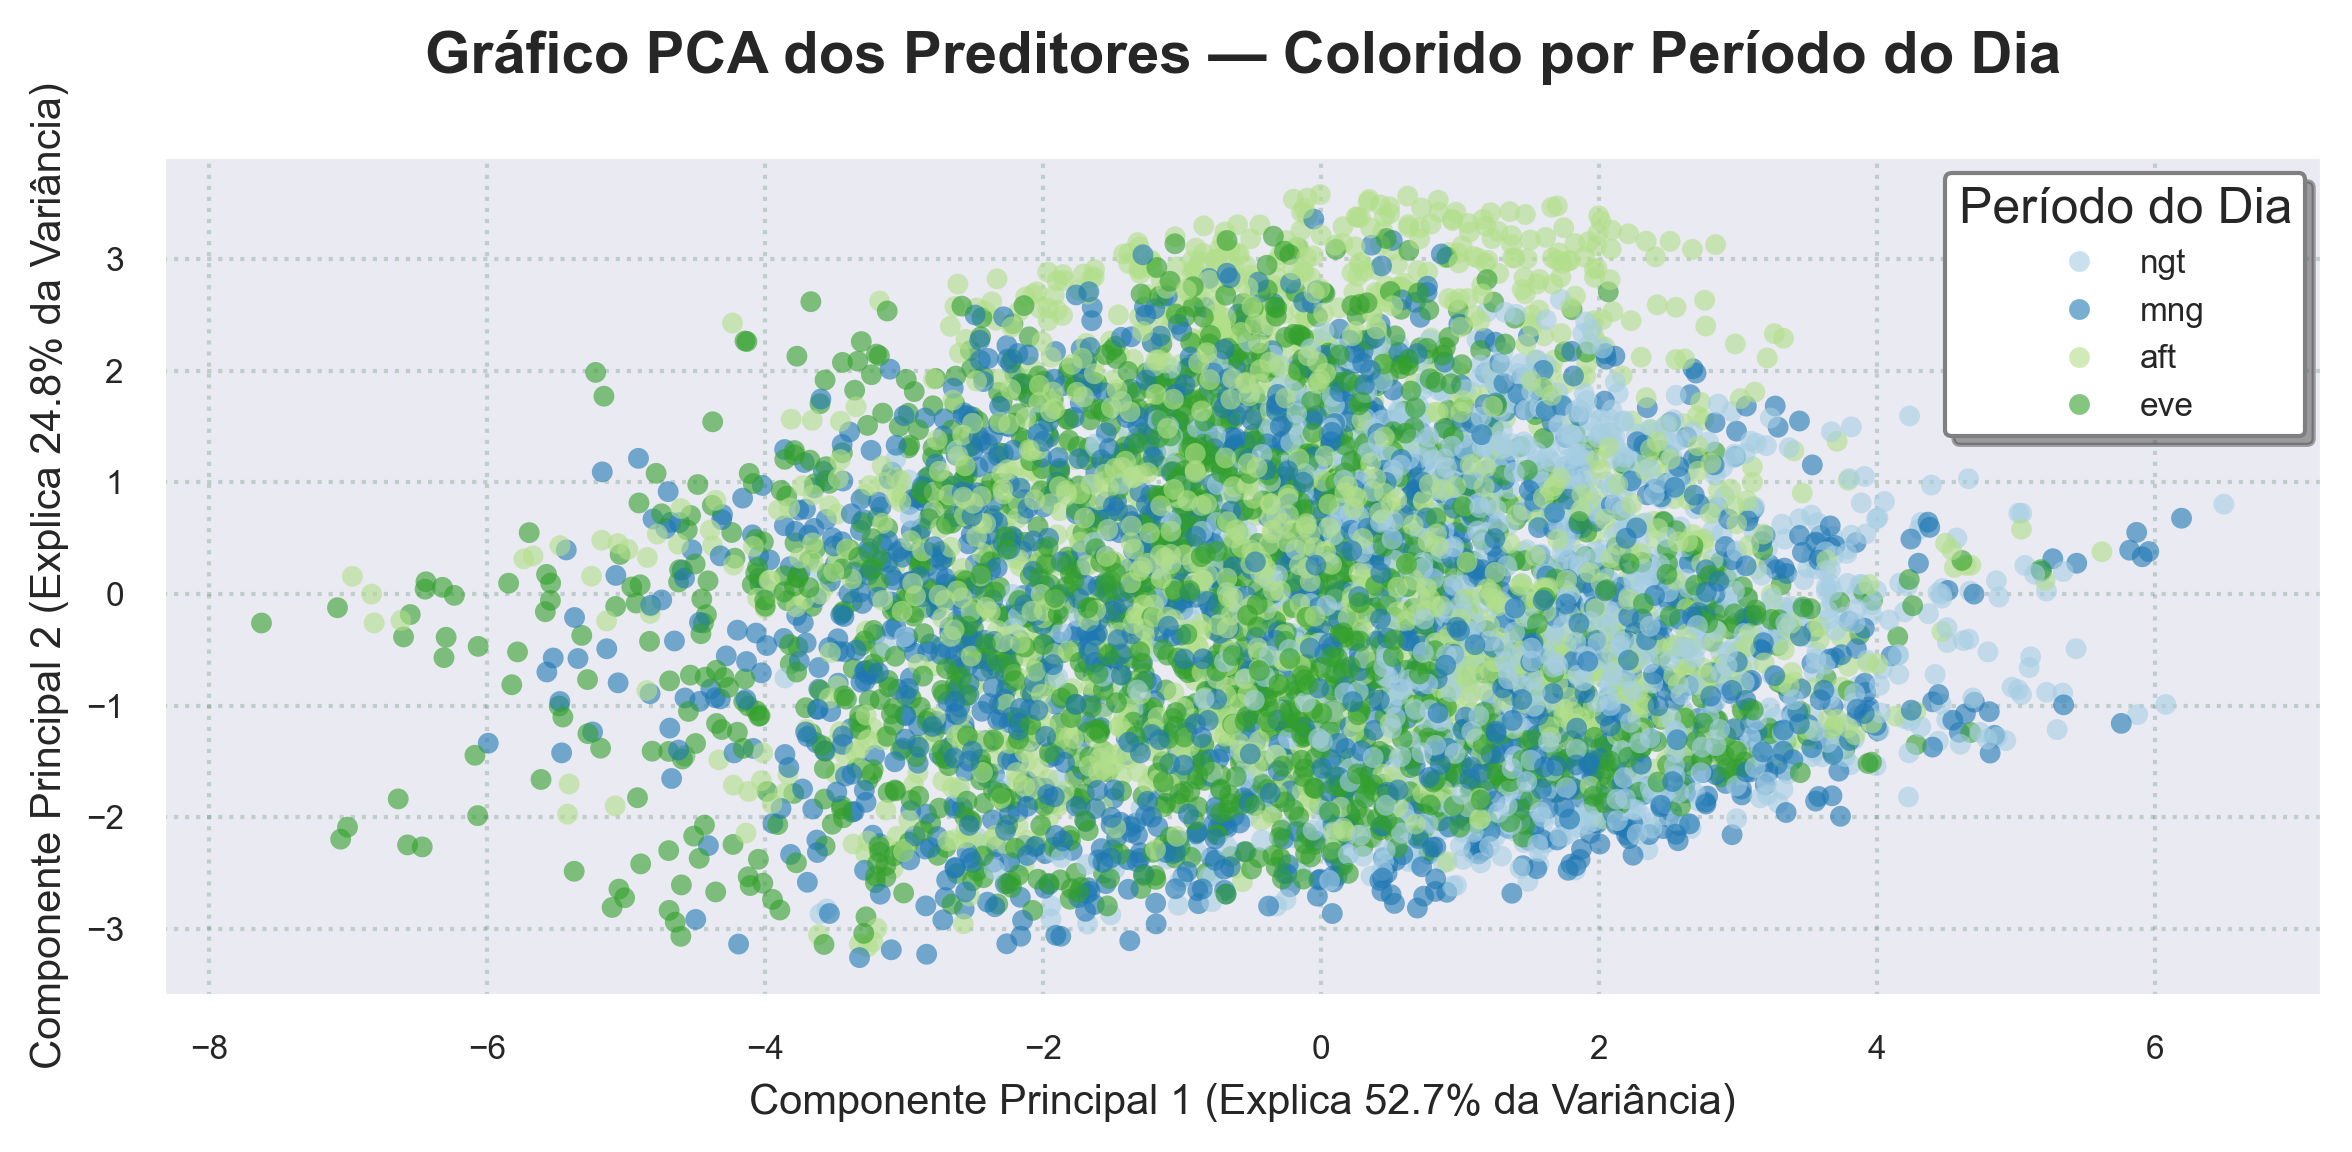
\includegraphics[width=0.95\linewidth]{figures/pca_2d_scatterplot_by_dayperiod.png}
    \caption{Dispersão em duas dimensões (PC1 e PC2), colorida por período do dia. Observa-se separabilidade parcial entre períodos.}
    \label{fig:pca2d}
\end{figure}

\subsection{Contagem de \emph{outliers} por variável (limiar \( |z|>3 \))}
A Tabela~\ref{tab:outliers} sumariza a contagem de \emph{outliers} por variável segundo o critério \( |z|>3 \).

\begin{table}[htbp]
    \centering
    \caption{Contagem de \emph{outliers} por variável sob \( |z|>3 \).}
    \label{tab:outliers}
    \begin{tabular}{lr}
        \hline
        \textbf{Variável} & \textbf{Contagem} \\
        \hline
        \texttt{NOx(GT)\_z}         & 118 \\
        \texttt{NOx(GT)}            & 118 \\
        \texttt{CO(GT)\_z}          & 87 \\
        \texttt{CO(GT)}             & 87 \\
        \texttt{PT08.S3(NOx)}       & 87 \\
        \texttt{C6H6(GT)}           & 85 \\
        \texttt{C6H6(GT)\_z}        & 85 \\
        \texttt{pollution\_index}   & 71 \\
        \texttt{PT08.S1(CO)}        & 41 \\
        \texttt{NO2(GT)}            & 36 \\
        \texttt{NO2(GT)\_z}         & 36 \\
        \texttt{PT08.S5(O3)}        & 27 \\
        \texttt{PT08.S2(NMHC)}      & 27 \\
        \texttt{PT08.S4(NO2)}       & 27 \\
        \texttt{NMHC(GT)}           & 9 \\
        \texttt{T}                  & 2 \\
        \texttt{AH}                 & 0 \\
        \texttt{RH}                 & 0 \\
        \hline
    \end{tabular}
\end{table}

\noindent\textbf{Leitura:} \texttt{NOx(GT)} lidera em \emph{outliers}, seguido de \texttt{CO(GT)} e \texttt{PT08.S3(NOx)}; meteorológicas (\texttt{T}, \texttt{RH}, \texttt{AH}) exibem raríssimos ou nenhum \emph{outlier}. Isso corrobora que PC1 concentra episódios de alta intensidade nos sensores/poluentes, enquanto PC2 se mantém mais estável (controle meteorológico).

\subsection{Implicações para modelagem}
\begin{itemize}
    \item \textbf{Redução de dimensionalidade:} 2--3 componentes já resumem \( \approx 78\% \) a \( \approx 92\% \) da variância dos preditores, reduzindo colinearidade.
    \item \textbf{Modelos candidatos:} PCR/PLS são apropriados; \emph{ridge}/\emph{lasso} também mitigam multicolinearidade e \emph{outliers} moderados; considerar transformações (p.ex., \(\log(1+x)\)) para variáveis altamente assimétricas.
    \item \textbf{Correção ambiental:} incluir \texttt{T}, \texttt{RH}, \texttt{AH} (ou PC2) e interações sensor×meteorologia melhora calibração.
    \item \textbf{Tempo do dia:} usar codificação contínua de hora (seno/cosseno ou \emph{splines}) auxilia a capturar a variação gradual vista em PC2.
\end{itemize}
